\subsection{Spatial Dependence}\label{sec:spatialresults}

Both indices are spatially clustered (Table~\ref{tab:moran}). Under rook contiguity, Moran's $I$ for DFA ranges from 0.239 to 0.314 and for RCD from 0.377 to 0.427, and the null of no autocorrelation is rejected at the 5\% level or better in every year. Under inverse-squared-distance weights the RCD clustering persists (0.117 to 0.175) while the DFA statistic falls to between 0.017 and 0.068 and is only marginally significant in 2013 and 2021. Digital factors therefore concentrate in adjacent provinces---coastal agglomerations and contiguous western blocks---rather than decaying smoothly with distance. The clustering survives the within transformation: after province demeaning, mean Moran's $I$ is 0.323 for DFA and 0.244 for RCD, positive in eight of nine years.

Figure~\ref{fig:lisa} maps the local clusters. Shanghai and Jiangsu are high--high for both indices in both years, Tianjin is high--high for DFA, and Zhejiang joins both clusters by 2021. The low--low block in the west consolidates: for RCD it grows from seven provinces in 2013 to nine in 2021, adding Inner Mongolia, Ningxia, and Shaanxi while Guizhou drops out. Hainan is a low--high outlier throughout. Beijing is high in both indices but is not classified as a cluster because its neighbours are much poorer; it is a single-province peak rather than part of an agglomeration.

\begin{table}[H]
\caption{Global Moran's $I$ for DFA and RCD.}\label{tab:moran}
\begin{threeparttable}
\footnotesize
\begin{tabular}{llrrrrrrrr}
\toprule
Index & W & \multicolumn{8}{c}{Global Moran's $I$ by year} \\
\cmidrule(lr){3-10}
 & & 2013 & 2014 & 2015 & 2016 & 2017 & 2018 & 2019 & 2021 \\
\midrule
DFA & Rook contiguity & 0.249** & 0.249** & 0.240** & 0.239** & 0.256** & 0.269** & 0.284** & 0.314** \\
DFA & Inverse distance & 0.049* & 0.042 & 0.017 & 0.029 & 0.036 & 0.032 & 0.041 & 0.068* \\
\midrule
RCD & Rook contiguity & 0.413*** & 0.410*** & 0.393*** & 0.377*** & 0.384*** & 0.387*** & 0.377*** & 0.427*** \\
RCD & Inverse distance & 0.175** & 0.173*** & 0.135** & 0.124** & 0.129** & 0.133** & 0.117** & 0.168** \\
\bottomrule
\end{tabular}
\begin{tablenotes}
\footnotesize
\item Notes: Inference is based on 999 random permutations of the cross-section within each year. $^{***}p<0.01$, $^{**}p<0.05$, $^{*}p<0.10$. Rook contiguity is row-standardized; Hainan is linked to Guangdong because it has no land neighbour. The inverse-distance weights use the squared reciprocal of the distance between provincial centroids.
\end{tablenotes}
\end{threeparttable}
\end{table}

\begin{figure}[H]
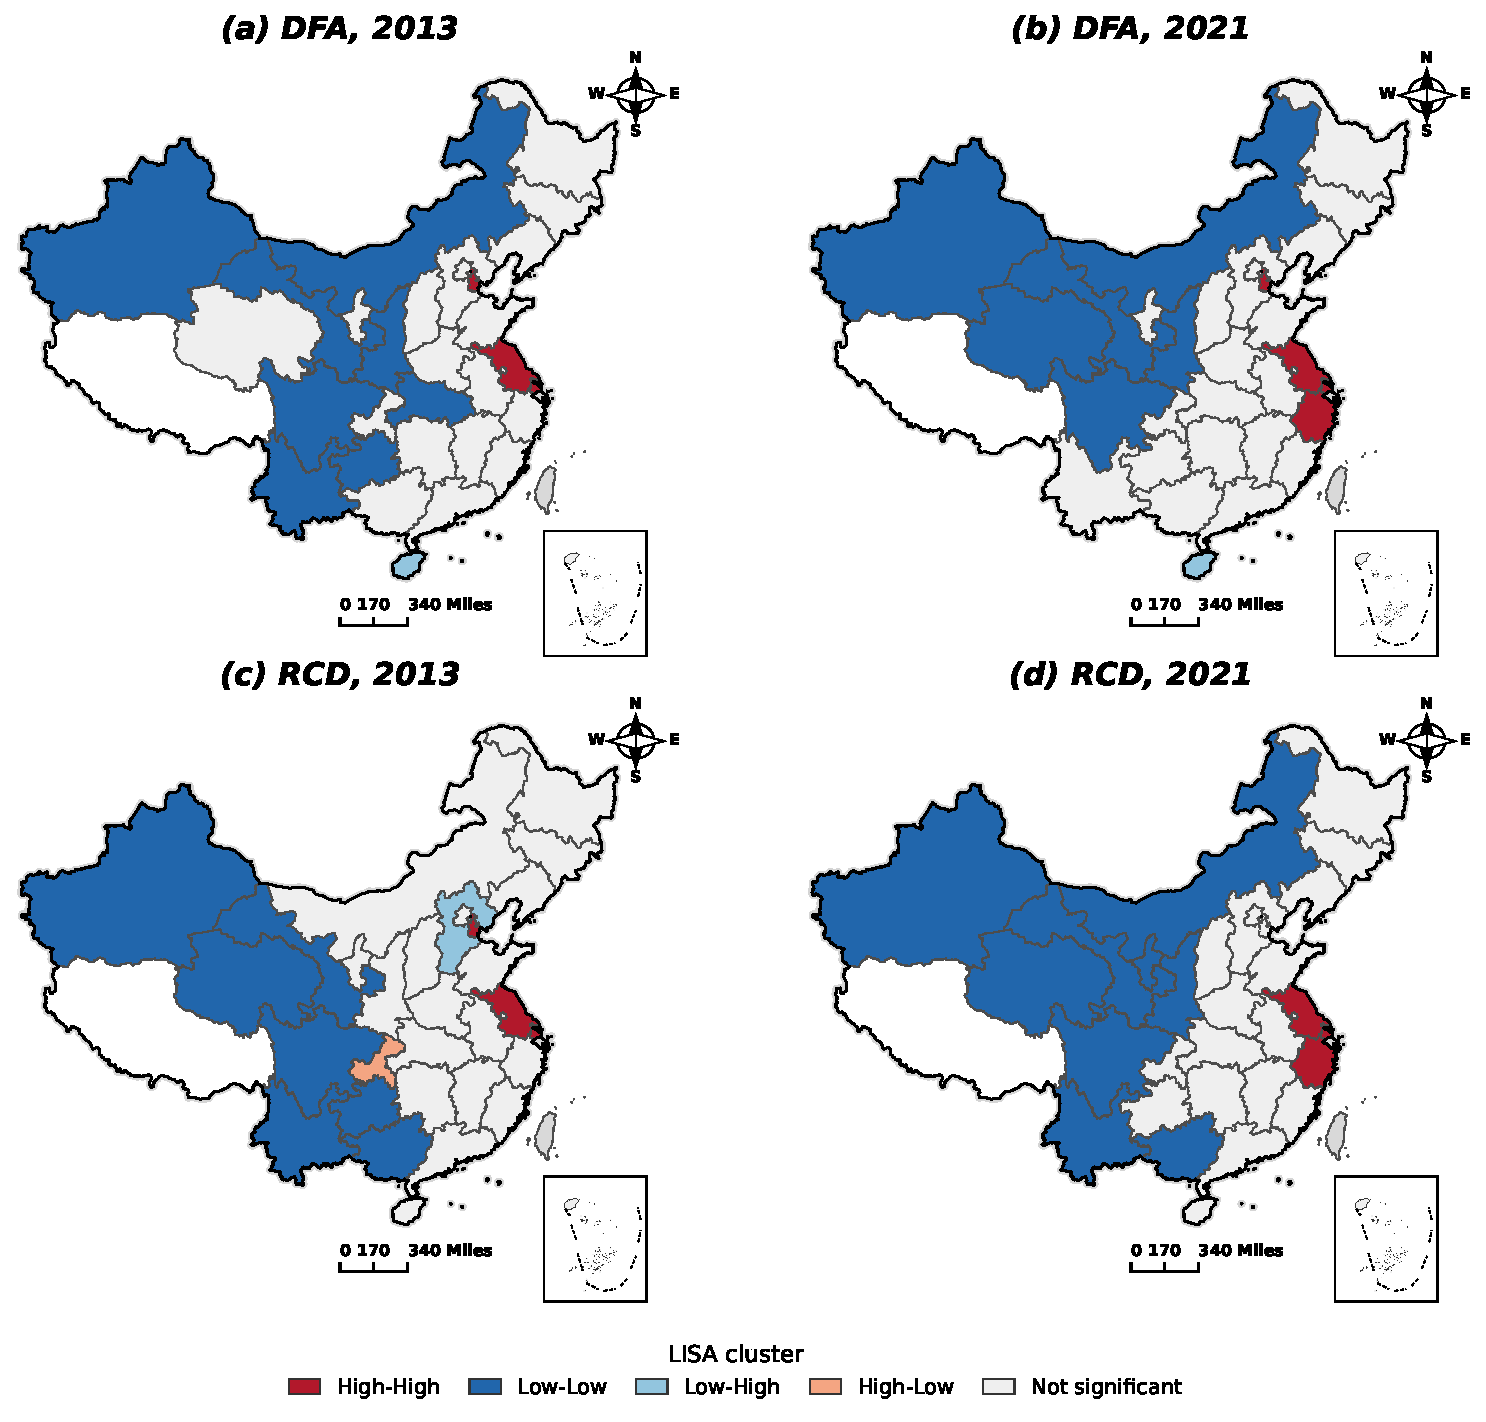
\includegraphics[width=\textwidth]{figures/fig_lisa_map.pdf}
\caption{Local Moran clusters (LISA) for DFA and RCD, 2013 and 2021. A province is classified as a cluster when the pseudo $p$-value from 999 permutations is below 0.10; the remaining provinces are shown as not significant. Tibet is not in the estimation sample and is left blank.}\label{fig:lisa}
\end{figure}

Table~\ref{tab:spatialthreshold} asks whether the threshold survives these patterns. The spatial autoregressive specification places the threshold at 10.583, essentially the baseline value of 10.589, and estimates $\rho=0.580$; the regime coefficients fall to 0.169 and 0.274, the bootstrap $p$-value for the break rises to 0.143, and the implied total effects are 0.402 and 0.652. The spatial error specification places the threshold at 11.181 (about CNY 71{,}900) and estimates a declining slope (0.615 against 0.550). The SLX row is reported for completeness only: the coefficient on neighbouring DFA cannot be separated from the own-province coefficient because the two are correlated at 0.979 after the within transformation.

The location of the threshold is therefore stable when the outcome is allowed to depend on neighbouring outcomes, and the positive association holds in both regimes under every specification. The size of the break is not stable, ranging from about 0.17 in the baseline to roughly zero in the spatial error model. We read the threshold as a development gradient rather than a sharp structural break.

\begin{table}[H]
\caption{Threshold estimates with spatial controls.}\label{tab:spatialthreshold}
\begin{threeparttable}
\footnotesize
\begin{tabular}{lcccccc}
\toprule
Model & $\hat{\gamma}$ & Bootstrap $p$ & Low regime & High regime & Spatial parameter & $N$ \\
\midrule
Baseline & 10.589 & 0.003 & 0.506*** (0.058) & 0.677*** (0.069) &  & 270 \\
SLX\textsuperscript{a} & 10.589 & 0.030 & 0.133 (0.154) & 0.275* (0.158) &  & 270 \\
Spatial error & 11.181 & 0.027 & 0.615*** (0.111) & 0.550*** (0.110) & 0.720 & 270 \\
Spatial autoregressive & 10.583 & 0.143 & 0.169*** (0.055) & 0.274*** (0.060) & 0.580 & 270 \\
\midrule
\multicolumn{3}{l}{\textit{Panel B: Effects in the SAR model}} & \textit{Direct} & \textit{Indirect} & \textit{Total} & \\
\midrule
Low regime & & & 0.188 & 0.214 & 0.402 & \\
High regime & & & 0.305 & 0.347 & 0.652 & \\
\bottomrule
\end{tabular}
\begin{tablenotes}
\footnotesize
\item Notes: All models include province fixed effects and the full control set, and the threshold variable is log GDP per capita. The bootstrap $p$-value is based on 300 cluster wild bootstrap replications and tests the null of a single linear regime; for the spatial error and spatial autoregressive models the bootstrap is conditional on the estimated spatial parameter. The spatial parameter is $\lambda$ for the spatial error model and $\rho$ for the spatial autoregressive model. Panel B reports the direct, indirect, and total effects of DFA in the spatial autoregressive model, computed from $(I-\rho W)^{-1}$ with row-standardized weights. The SLX specification (row 2) is not identified. Standard errors clustered by province are in parentheses. $^{***}p<0.01$, $^{**}p<0.05$, $^{*}p<0.10$.
\end{tablenotes}
\end{threeparttable}
\end{table}

\subsection{Which Digital Factor Matters?}\label{sec:subdims}

Table~\ref{tab:subdims} enters the four normalized dimension scores separately and jointly, and repeats the threshold model for each dimension. Digital finance is the only dimension with an independent association: 0.134 (p $<$ 0.05) on its own and 0.151 (p $<$ 0.01) when entered jointly with the other three, which are indistinguishable from zero. Digital infrastructure (0.057) and digital industry (0.069) are positive but imprecise, and digital human capital is negative ($-0.173$) and imprecise. Measured against the three-dimension outcome, financial inclusion is doing much of the work.

The dimensions also have different threshold patterns. Digital infrastructure is positive in both regimes but larger below the threshold (0.587 against 0.278), consistent with diminishing returns to basic connectivity. Digital industry and digital human capital switch from negative below the threshold to positive above it ($-0.250$ to 0.113 and $-0.341$ to 0.102), the pattern an absorptive-capacity argument predicts. Digital finance is positive in both regimes and slightly larger above (0.168 to 0.234). The rising pattern of the composite index is the net of these four, which is why it is milder than the individual breaks for industry and human capital.

The negative low-regime coefficients should not be read as evidence that digital industry or digital skills harm lagging provinces. They are more plausibly a failure of these factors to translate into coordination without the complementary conditions that define the high regime. The low-income regime contains only 66 observations, so these slopes are imprecise.

\begin{table}[H]
\caption{Digital factor dimensions: separate, joint, and threshold estimates.}\label{tab:subdims}
\small
\begin{tabular}{lcccccc}
\toprule
\multicolumn{7}{l}{\textit{Panel A: Two-way fixed effects, each dimension entered separately and jointly}} \\
\midrule
 & \multicolumn{2}{c}{Separate} & \multicolumn{2}{c}{Joint} & \multicolumn{2}{c}{Threshold model} \\
\cmidrule(lr){2-3}\cmidrule(lr){4-5}\cmidrule(lr){6-7}
Dimension & Coefficient & $p$ & Coefficient & $p$ & Low regime & High regime \\
\midrule
Digital infrastructure & 0.044 & 0.539 & 0.057 & 0.460 & 0.587 & 0.278 \\
Digital industry & 0.069 & 0.385 & 0.069 & 0.320 & -0.250 & 0.113 \\
Digital finance & 0.134** & 0.012 & 0.151*** & 0.003 & 0.168 & 0.234 \\
Digital human capital & -0.113 & 0.270 & -0.173 & 0.142 & -0.341 & 0.102 \\
\bottomrule
\end{tabular}

\vspace{6pt}
\begin{tabular}{lcccc}
\toprule
Dimension & $\hat{\gamma}$ & $F$ & Bootstrap $p$ & $N$ \\
\midrule
Digital infrastructure & 11.178 & 39.70 & 0.005 & 270 \\
Digital industry & 10.586 & 47.53 & <0.005 & 270 \\
Digital finance & 10.586 & 28.05 & 0.005 & 270 \\
Digital human capital & 10.586 & 61.75 & <0.005 & 270 \\
\bottomrule
\end{tabular}

\vspace{3pt}
\parbox{\textwidth}{\footnotesize\textit{Notes:} Each dimension score is the entropy-weighted within-dimension index, min--max normalized over the panel. In the upper table, columns (1) and (2) report each dimension entered separately, columns (3) and (4) report all four dimensions entered jointly, and columns (5) and (6) report the regime-specific coefficients from a separate threshold model for each dimension. The lower table reports the estimated threshold and the bootstrap $p$-value for each dimension. All models include province and year fixed effects (threshold models: province fixed effects only) and the full control set. Standard errors clustered by province. $^{***}p<0.01$, $^{**}p<0.05$, $^{*}p<0.10$.}
\end{table}

\subsection{Specification and Identification Checks}\label{sec:identification}

Panel A of Table~\ref{tab:idchecks} reports Oster (2019) bounds, which ask how strong selection on unobservables would have to be, relative to the observed controls, to drive the DFA coefficient to zero. Under two-way fixed effects the coefficient moves from 0.277 without controls to 0.241 with them, and the bias-adjusted value at $\delta=1$ is 0.213. The value of $\delta$ required to reach zero is 8.58, against the benchmark of 1 that Oster suggests. Under province fixed effects the required value is 27.4; adding the three additional controls lowers the coefficient to 0.213 and the required value to 1.74, still above the benchmark.

Panel B reports a randomisation placebo. If the threshold reflected the true development ordering, reassigning income levels across provinces within each year should destroy it. Over 499 permutations the mean Hansen $F$ is 5.85 and its 95th percentile is 12.00, against an observed value of 26.74 (p $=$ 0.002), and the permuted threshold estimates are dispersed (median 10.978, interquartile range 10.604 to 11.276). The threshold is not an artefact of searching over a spatially clustered variable.

A continuous moderation specification points the other way. Interacting DFA with log GDP per capita gives a coefficient of 0.012 (p $=$ 0.90), and with financial development $-0.002$ (p $=$ 0.75) (Table~\ref{tab:interaction}). A regime shift and a smooth gradient are different hypotheses, and the nonlinearity in this paper rests on the threshold parameterisation.

We do not report an instrumental-variable or dynamic-panel threshold estimate. Such estimators require an external instrument for DFA---historical telephone penetration, terrain ruggedness, or distance to the backbone network---none of which is available here, and we do not construct a pseudo-instrument from the indicators that enter the index. The estimates are therefore conditional associations, robust to the observed confounders and to spatial dependence. The formal mediation test in Appendix~\ref{app:mechanisms} points the same way: the bootstrap intervals for the indirect effects include zero in both regimes.

\begin{table}[H]
\caption{Oster bounds and randomisation inference.}\label{tab:idchecks}
\small
\begin{tabular}{lcccc}
\toprule
\multicolumn{5}{l}{\textit{Panel A: Oster (2019) bounds}} \\
\midrule
Specification & $\tilde{\beta}$ & $R^2$ & $\beta^*$ & $\delta^*$ \\
\midrule
Two-way FE, baseline controls & 0.241 & 0.171 & 0.213 & 8.58 \\
Province FE, baseline controls & 0.689 & 0.895 & 0.664 & 27.40 \\
Two-way FE, additional controls & 0.213 & 0.184 & 0.090 & 1.74 \\
\midrule
\multicolumn{5}{l}{\textit{Panel B: Randomisation inference for the threshold}} \\
\midrule
Observed $F$ & Mean & 95th pct. & $p$-value & Reps. \\
\midrule
26.74 & 5.85 & 12.00 & 0.002 & 499 \\
\bottomrule
\end{tabular}

\vspace{3pt}
\parbox{\textwidth}{\footnotesize\textit{Notes:} Panel A reports Oster (2019) bounds. $\tilde{\beta}$ is the coefficient of DFA with the full control set and $\beta^{*}$ is the bias-adjusted coefficient at $\delta=1$ with $R_{\max}=1.3\tilde{R}^{2}$ (capped at 1). $\delta^{*}$ is the degree of selection on unobservables, relative to selection on observables, that would be required to drive the coefficient to zero. Panel B permutes log GDP per capita across provinces within each year and re-estimates the threshold model 499 times; the $p$-value is the share of permuted $F$ statistics at least as large as the observed one.}
\end{table}
